\chapter{Начало разработки}

\section{Обзор микроконтроллеров}



\section{Среды разработки для STM32}




\section{Методы программной генерации сигнала}
	Основные методы цифровой генерации сигналов --- метод аппроксимации и табличный метод.
	
	Метод аппроксимации подразумевает собой вычисление отсчётов функции с заданным интервалом. В памяти хранятся только параметры сигнала. Поэтому данный метод позволяет затратить небольшой объём памяти, но его недостаток это затраты на вычисления, что ограничивает максимальную частоту сигнала.
	
	В табличном методе генерации сигналов предполагается, что заранее вычисленные отсчёты хранятся в памяти. То есть никаких вычислений не требуется и генерация сводится к тому, что в порт цифро-аналогового преобразователя нужно вывести ячейку по заданному адресу. Таким образом, время на формирование отсчёта становится меньше и появляется возможность генерировать сигнал с более высокой частотой. Недостатком же является большие затраты памяти.
	
	Будем рассматривать табличный метод синтеза. Для начала потребуется таблица отсчётов, чтобы её вычислить используем готовый инструмент.
	
	\begin{figure}[H]
    \centering
    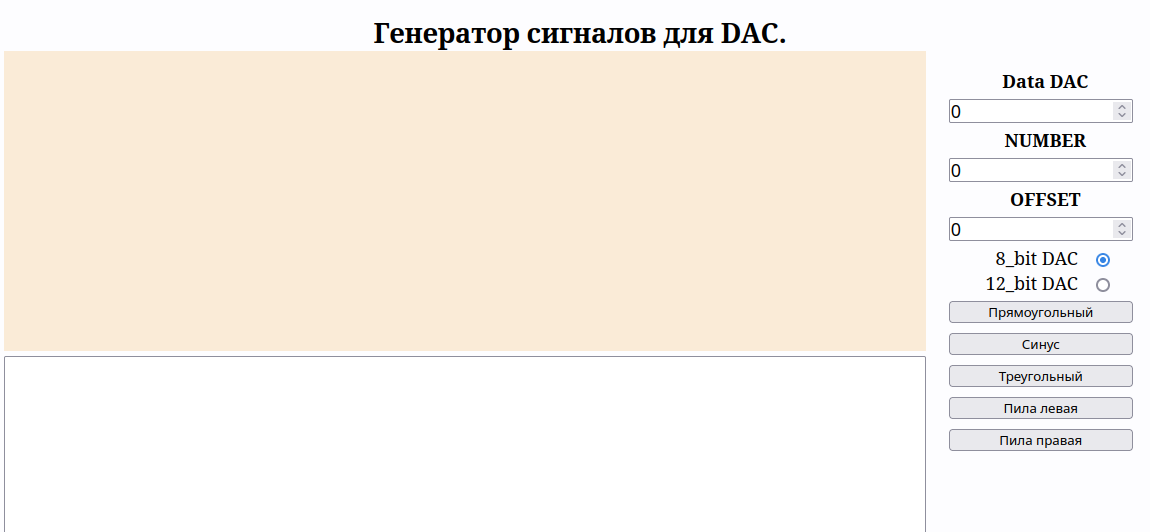
\includegraphics[width=1\textwidth]{../image/lut_prog.png}
    \caption{Программа для вычисления значений сигнала.}
	\end{figure}
	
	У таблицы есть 4 параметра:
	\begin{enumerate}
		\item Разрядность ЦАП: 8 или 12 бит.
		\item Максимальное значение.
		\item Количество значений.
		\item Смещение от нуля.
	\end{enumerate}
	
	Использовать мы будем 12-битные значения в количестве 256 чисел. Максимальное значение амплитуды сигнала может быть 4095, но так как для улучшения генерации будет задействован встроенный в цифро-аналоговый преобразователь выходной буфер, то он будет срезать сигнал сверху и снизу на 0.2В, поэтому значения тоже следует срезать на эту же величину для корректной генерации.
	
	В документе от ST про работу с цифро-аналоговым преобразователем есть формула для расчета выходного напряжения.
	
	$DAC_{output} = V_{REF}*\dfrac{DOR}{DAC_{MaxDigitalValue} + 1}$, где DOR --- цифровое значение.
	
	Нам нужно найти какое значение соответствует напряжению 0.2В. Выразим DOR и подставим имеющиеся значения.
	
	$DOR = \dfrac{V_{REF}}{DOR}*DAC_{MaxDigitalValue} + 1 = \dfrac{3.3}{0.2}*(4095+1) = 248$
	
	Укажем смещение от нуля 248, а максимальное значение 4095 меньше на 248, то есть 3847 и сгенеририуем таблицу отсчётов для синусоиды. 
	
	\begin{figure}[H]
    \centering
    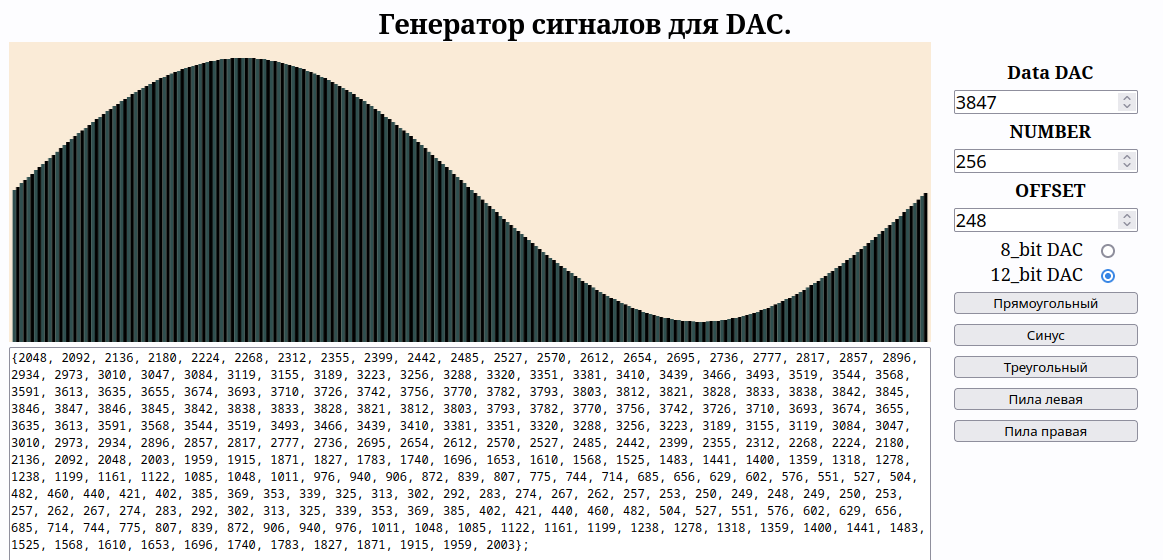
\includegraphics[width=1\textwidth]{../image/lut.png}
    \caption{Вычисление таблицы сигнала.}
	\end{figure}
	
	Теперь у нас есть данные для генерации сигнала, но теперь нужно продумать как передавать их в цап и как вообще работать с цапом.